\documentclass[11pt]{article}

\usepackage[utf8]{inputenc}
\usepackage{acl2015}
%\usepackage{url}
\usepackage{natbib}
\usepackage{graphicx}
\usepackage{multicol}
\usepackage{hyperref}
\usepackage{threeparttable}
\usepackage{algorithm2e}

\title{This Time With Feeling: Sentiment to ML Headlines}

\author{Ben Arnoldy \\
  University of California, Berkeley \\
  {\tt arnoldyb@berkeley.edu} \\\And
  Mark Paluta \\
  University of California, Berkeley \\
  {\tt mpaluta@berkeley.edu} \\}
  
\date{July 2019}

\begin{document}

\maketitle

\begin{abstract}
    
\end{abstract}

\section{Introduction}
The art of good headline writing is not as simple as summarizing relevant details; it requires wit, originality, and a tone that matches the piece. Algorithms have made improvements in summarization, but still struggle with these more nuanced elements. Despite this shortcoming, algorithms could still be useful to an editor, suggesting a number of possible headlines to provide inspiration or for the editor to refine and synthesize into a final product. We propose an incremental improvement in automatic headline generation by incorporating tonal bias to match the underlying content.

\section{Background}
Headline generation is primarily approached as a single-document summarization task. The nature of headlines makes them relatively more difficult to produce with machine learning than typical document summaries. First, headlines tend to be shorter than the average sentence, requiring greater concision than typical ML summaries of one or more sentences. Additionally, they are often written in a short-hand style different from the body text, making extractive summarization theoretically less suitable than the more challenging task of abstractive summarization. 

Current methods of summarization involve an encoder-decoder architecture \citep{rush2015neural} with a ROUGE evaluation metric \cite{Ayana2017}. ROUGE is a recall-oriented metric to score a generated summary against a reference summary \cite{lin-2004-rouge}. Specific variants include ROUGE-N, scoring the number of common N-grams, and ROUGE-L, scoring the longest common subsequence. Recent refinements to headline generation include adversarial reward systems to combat repetition \cite{DBLP:journals/corr/abs-1902-07110} and applying state-of-the-art Transformer algorithms \cite{DBLP:journals/corr/abs-1901-07786}.

While most work on headline generation focuses exclusively on summarization, two recent papers in other summarization domains explored efforts to add desired sentiment. One naive approach from Chaudhari et al \cite{DBLP:journals/corr/abs-1802-09426} preprocessed sentences in the body of the corpus to generate sentence-level sentiment scores that characterize the emotional tone of the text. Sentences that did not match the desired sentiment polarity (positive or negative) were dropped before training the summarization model. Another more elaborate approach from Hu et al \cite{DBLP:journals/corr/HuYLSX17} to produce customer review summaries added a discriminator to evaluate the sentiment of generated summaries, looping back to the generator to optimize on this additional criterion. 


\begin{figure*}
  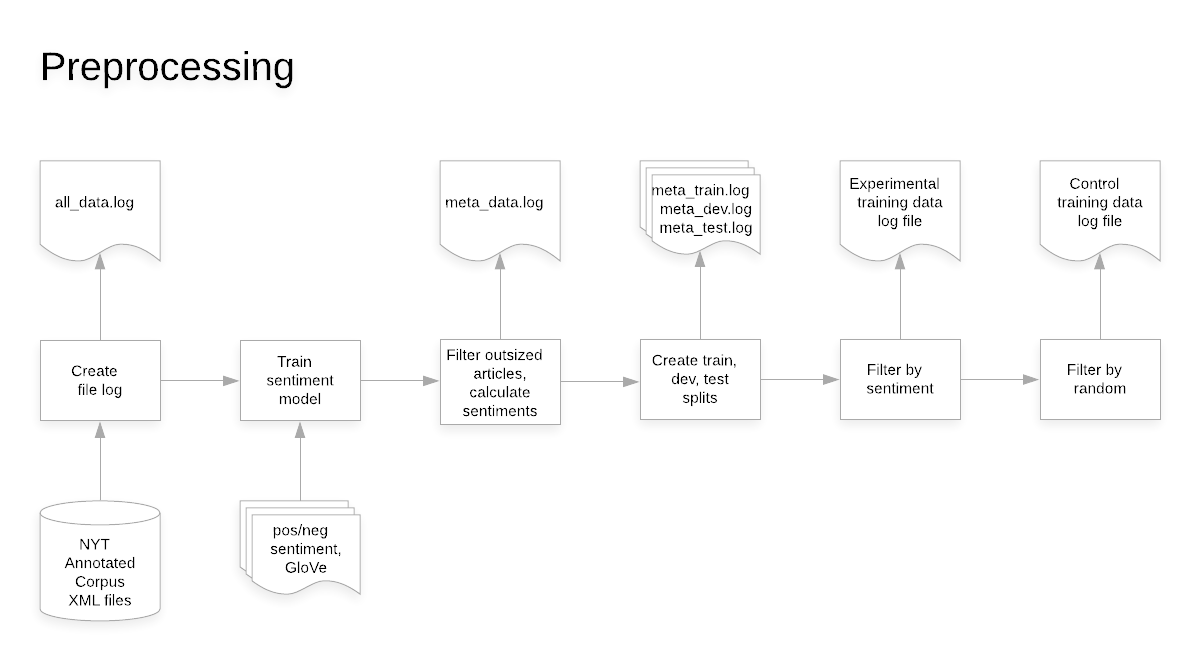
\includegraphics[width=\textwidth,height=7cm]{Headgen_prep.png}
  \caption{Preprocessing workflow}
\end{figure*}

\section{Methodology}

\subsection{Objective}
We build a Universal Transformer architecture, initially basing our algorithm off of that of Gavrilov et al \cite{DBLP:journals/corr/abs-1901-07786}, but adding sentiment into the model in the spirit of Chaudhari   \cite{DBLP:journals/corr/abs-1802-09426} and Hu \cite{DBLP:journals/corr/HuYLSX17}. To test the effectiveness of adding sentiment, we train an experimental and a control model.
The experimental model trains on the subset of the train dataset where the headline and the summary (i.e. lead) have the same sentiment polarity. This requirement results in a reduction in this model's training set from XXXXXXXX articles to 749,745. To ensure that the control model trains on a comparable amount of data, we reduce the control dataset by randomly dropping articles by the same amount, XXXXXX down to 749,745. 
With this naive approach modeled on Chaudari\cite{DBLP:journals/corr/abs-1802-09426}, we aim to get an early indication of whether the inclusion of sentiment in the headline generation task could improve ROUGE scores and result in generated headlines that better reflect the sentiment of the input text. Our hypothesis is that the experimental model will show a small gain in traditional ROUGE scores and improved scores on sentiment matching metrics over the control model. 
/////////ALTERNATIVE LANGUAGEWe use sentiment-based preprocessing to downsample examples where sentiment between body and headline matches poorly, thereby training largely on examples where body and headline match well. Our objective is to increase the sentiment match between an article's headline and body while simultaneously obtaining similar ROUGE scores.////////////

\subsection{Workflow}

The workflow we defined to preprocess, train, and evaluate our data can be seen in algorithm \ref{alg:1}. Note that the algorithm can be parallelized across three virtual machines for the three filtering options.

Suggesting we remove this in favor of your diagram

\begin{algorithm}[H]
\SetAlgoLined
 \For{filtering in (none, sentiment, random)}{
    1: preprocessing and metadata generation\;
    2: randomize train-dev-test split\;
    3: \If{filtering = sentiment}{
        4: sentiment-based downsampling\;}
    5: \If{filtering = random}{
        6: random downsampling\;}
    7: train on training set\;
    8: decode dev or test set\;
    9: score ROUGE metrics
    10: score sentiment metric\;
 }
 \caption{End-to-end pipeline}
\label{alg:1}
\end{algorithm}

\subsection{Universal Transformer Architecture}
We use an encoder-decoder architecture, AdamW optimizer, and the set of specific hyperparameters outlined by Gavrilov et al \cite{DBLP:journals/corr/abs-1901-07786} as our baseline. Noteworthy parameters are listed in Table \ref{table:1}. A diagram of the architecture can be viewed in Figure \ref{figure:1}.

\begin{table}[h!]
\centering
\begin{tabular}{|c | c|} 
 \hline
 Hyperparameter & Value \\ [0.5ex] 
 \hline
 Hidden layer size & 1024 \\ 
 Filter size & 4096 \\
 Heads of attention & 8 \\
 Layer preprocess sequence & None \\
 Layer postprocess sequence & dropout \\
 & $\rightarrow$ add $\rightarrow$ \\
 & normalize \\
 Postprocess dropout & 0.3 \\
 Encoder layers & 4 \\
 Decoder layers & 4 \\
 Learning rate warmup steps & 4000 \\ [1ex]
 \hline
\end{tabular}
\caption{Gavrilov's Hyperparameters}
\label{table:1}
\end{table}

\begin{table}[h!]
\centering
\begin{tabular}{|c | c|} 
 \hline
 Hyperparameter & Value \\ [0.5ex] 
 \hline
 Hidden layer size & 1024 \\ 
 Filter size & 4096 \\
 Heads of attention & 16 \\
 Layer preprocess sequence & normalize \\
 Layer postprocess sequence & dropout \\
 & $\rightarrow$ add $\rightarrow$ \\
 Preprocess dropout & 0.3 \\
 Encoder layers & 0 \\
 Decoder layers & 0 \\
 Learning rate warmup steps & 8000 \\ [1ex]
 \hline
\end{tabular}
\caption{T2T's _base Hyperparameters}
\label{table:1}
\end{table}

\subsection{corpus}
We use the \href{https://catalog.ldc.upenn.edu/LDC2008T19}{New York Times annotated corpus} to match Gavrilov. This contains 1.8 million New York Times articles spanning from 1987 to 2006. Like Gavrilov, we filtered out obituaries and articles with wordcount < 20 or > 2000 and headline length < 3 or > 15. We were left with XXXXXXX articles, which we then split along 70:10:20 proportions into train, dev, and test datasets. We also remove duplicative first paragraphs that occur in many of the articles. 

\subsection{Sentiment analysis}
We use a positive-negative polarity function as most research on sentiment is a simple positive-negative scale and we wish to leverage existing work. Following a model annotated by Speer\cite{RacistAI}, we take Liu's opinion lexicon\cite{Hu:2004:MSC:1014052.1014073} -- a list of around 6,800 words that are labeled either positive or negative -- and embed the lexicon's words in pre-trained GloVe embeddings. These embeddings and their [0,1] labels are used to train a logistic regression model that returns the log probability of a new word being positive and the log probability of it being negative. The negative probability is subtracted from the positive to arrive at a score; positive scores indicate positive associations and vice versa. To score an entire headline, we sum the individual scores of all the words in the headline and take an average. We construct a filter to remove articles where the polarity of the headline and its short summary differ, as shown in figure XXX ///write it as an xor///.

\begin{figure*}
  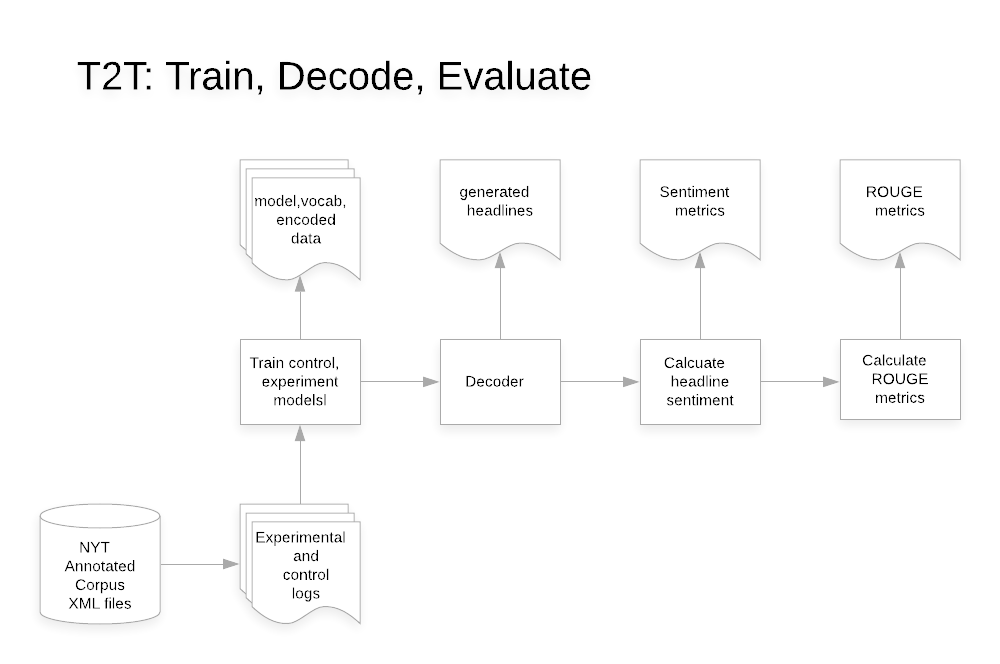
\includegraphics[width=\textwidth,height=7cm]{Headgen_train.png}
  \caption{Train, decode, evaluate workflow}
\end{figure*}

\subsection{Evaluation}
To test the quality of generated headlines, we ran the top portion of the body text in all of the test dataset articles through the decoder to generate headlines to evaluate the quality of the sentiment-filtered model and the control model. Our evaluation included both the standard ROUGE metrics used for summarization tasks as well as two measures of sentiment we designed. 
To compare the two models' performance on sentiment, we first calculate the percentage of generated headlines that match the polarity of the input body text. This percentage, which captures each model's ability to generate headlines that fit the sentiment of the their articles, is calculated as an f1-score where the headline's sentiment is the prediction for the true sentiment of the body. We expect that the preprocess filtering by sentiment will result in a trained model that produces higher f1-scores. Second, we subtract the difference in the predicted headline sentiment from the label headline sentiment and take an average across the dataset. This metric captures how well the models are able to generate headlines that match the sentiment of the label headlines. We expect that the experimental model will generate a smaller average sentiment differential than the control model, indicating a better sentiment match between predicted and label headlines.  
\subsection{Implementation}
Specifically, we chose to work with the package \href{https://github.com/tensorflow/tensor2tensor}{\texttt{tensor2tensor}}. This package was developed by the Google Brain team and is designed for furthering research on a variety of natural language processing problems\cite{vaswani-etal-2018-tensor2tensor}. We began by replicating the CNN/Daily Mail text summarization problem. We then adapted the architecture to accommodate a new problem of summarization, specifically headline generation rather than key point summarization, on the New York Times annotated corpus. The specific adaptations we made were as follows:

\begin{itemize}
    \item Prepare New York Times corpus for \texttt{tensor2tensor} ingestion by extracting filepath, headline, body, lede, word count, and other metadata, writing this data to a lot file, and performing a random train/dev/test split
    \item Define problem \texttt{Gavrilov} inheriting \texttt{Text2TextProblem}
    \item Apply a subword tokenizer to imitate Gavrilov et al's BPE tokenization
    \item Override a variety of default Universal Transformer hyperparameters as defined in Table \ref{table:1}
    \item Create optional sentiment preprocessing step
    \item Create optional random down-sampling step for control
\end{itemize}

\section{Results}
\subsection{Challenges with the decoder}

Due to the cutting-edge nature of \texttt{tensor2tensor} and limited documentation, the decoder posed a number of challenges for us. We experimented with adjusting the beam-size between 1 and 10, $\alpha$ (length normalization) between .01 and 100, and the \texttt{decode\_variable} parameter between 1 and 100, but regardless of settings we almost always got empty output from the decoder. We even adjusted from inputting 10 paragraphs to 3 and retrained entirely to try to downscope the problem and allow for faster convergence, but still encountered the problem. On rare occasions, we were able to get a few words repeated numerous times. We show one such example in Table \ref{table:3}. Note this is not actually an article from our data set, but was just an article selected from the front page of the New York Times.

\begin{table}[h!]
\centering
\begin{tiny}
\begin{tabular}{|p{7cm}|} 
 \hline
 \textbf{Input:} When Democratic Rep. Rashida Tlaib accused Republican Rep. Mark Meadows of racism earlier this year, one of his "best friends," House Oversight Committee chairman and Democratic Rep. Elijah Cummings immediately jumped to his defense. When Cummings was attacked on similar grounds by President Donald Trump over the weekend, it took a bit longer for Meadows to publicly repay the favor. On Saturday and Sunday, Trump went after Cummings on Twitter, calling the veteran Democratic lawmaker a "racist" and his district a "disgusting, rat and rodent infested mess." Trump's comments hung in the air for days, sparking yet another conversation about the President's race-focused rhetoric. Republicans largely stayed silent, including Meadows, whose warm relationship with Cummings prompted questions about his reticence to defend his friend. \\ [0.5ex] 
 \hline
 \textbf{Output:} Fatah Fatah Fatah Fatah Mitch Mitch Mitch Mitch Mitch Mitch Mitch Mitch Mitch Mitch Mitch Mitch Mitch Mitch Mitch Mitch Mitch Mitch Mitch Mitch Mitch Mitch Boys Boys Boys Boys Boys Boys Boys Boys Boys Boys Boys Fatah Fatah Fatah Fatah Fatah Boys Boys Boys Boys Boys Mitch Mitch Boys Boys Boys Mitch Mitch Mitch Fatah Fatah Fatah Boys Boys Mitch Mitch Mitch Mitch Mitch Mitch Boys Boys Boys Fatah Fatah Fatah Mitch Mitch Mitch Mitch Mitch Mitch Fatah Fatah Fatah Mitch Mitch Mitch Mitch Mitch Mitch Boys Boys Mitch Mitch Mitch Mitch Mitch Mitch Boys Boys Boys Boys Boys Boys Boys Boys Boys Boys Boys Boys Boys Boys Mitch Mitch Boys Boys Boys Boys Boys Mitch Mitch Boys Boys Fatah god god god god god god god god god god god Mitch Mitch Mitch god Mitch Mitch Mitch Mitch Mitch Mitch Mitch Mitch Mitch Mitch Mitch Mitch Mitch Mitch Mitch Mitch Mitch Mitch Mitch Mitch Mitch Mitch Mitch Mitch Mitch Mitch Mitch Mitch Mitch Mitch Mitch Mitch Mitch Mitch Mitch Mitch Mitch Mitch Mitch Mitch Mitch Mitch Mitch Mitch Mitch Mitch Mitch  \\ 
 \hline
\end{tabular}
\end{tiny}
\caption{Example Output}
\label{table:3}
\end{table}

It is unclear to us whether this indicates that the model is learning to associate topics like politics and Muslim Congresswoman Rashida Tlaib with Middle Eastern affairs (e.g. "Fatah", or "Mitch" perhaps referring to Mitch McConnell). It could also simply be coincidence.

We noticed that providing input via the command line "interactive decoder" was somewhat more likely to provide actual output than via reading a text file, which was perplexing. We also note that there are numerous open git issues with users reporting blank outputs in transformer architectures [several footnotes with links], it is unclear to us the reason for our largely blank decoder output. We see a few potential sources: a problem in our architecture construction, insufficient training time, or a bug within \texttt{tensor2tensor} based on the aforementioned apparent bugs. Based on the plausible output in at least one instance, we suspect the architecture is working appropriately.

\subsection{ROUGE and sentiment scores}
Given the decoder challenges, we abandoned the Universal Transformer hyperparameters outlined in Gavrilov and instead worked with preset Universal Transformer hyperparameters provided in Tensor2Tensor. This resulted in decoder output good enough to obtain meaningful ROUGE metrics and sentiment metrics. 
////SHOW A BETTER DECODER OUTPUT/////

 \texttt{tensor2tensor}. This is estimated by [maybe some math here]

\begin{table*}[h!]
\centering
\begin{small}
\begin{tabular}{|p{7cm}|p{.8cm}|p{.8cm}|p{.8cm}|p{.8cm}|p{.8cm}|p{.8cm}|p{1.3cm}|}
 \hline
 Model & R-1-f & R-1-r & R-2-f & R-2-r & R-L-f & R-L-r & Sentiment \\
 \hline
 Gavrilov Universal Transformer - unsmoothed & \textbf{26.86} & 25.33 & \textbf{13.48} & \textbf{13.01} & \textbf{24.84} & 24.38 & - \\ [0.5ex] 
 Gavrilov baseline (first sentence) & 11.64 & \textbf{34.67} & 2.28 & 7.43 & 7.19 & \textbf{31.39} & - \\ 
 Our baseline (first 8 words) & ? & ? & ? & ? & ? & ? & ? \\
 Our Universal Transformer - Sentiment-filtered & ? & ? & ? & ? & ? & ? & ? \\
 Our Universal Transformer - Randomly filtered & ? & ? & ? & ? & ? & ? & ? \\ [1ex]
 \hline
\end{tabular}
\end{small}
\caption{Results}
\label{table:4}
\end{table*}

\subsection{Resource considerations}

As we ran our algorithm on several different resource configurations, we decided to take the opportunity to record approximate computation times on various configurations to inform future resource requirements for future work, as some results were nonintuitive. Our approximate benchmarks can be seen in Table \ref{table:2}

\begin{table}[h!]
\begin{threeparttable}
\centering
\begin{small}
\begin{tabular}{|p{2cm}|p{2.2cm}|p{2cm}|} 
 \hline
 Task & Configuration & Approx. Computation Time \\ [0.5ex] 
 \hline\hline
 Vocab Generation & CPU-heavy^{1} & 5 hr 40 min \\ 
 Vocab Generation & Balanced^{2} & 40 min \\
 \hline
 One training step & CPU-heavy & 3.9 sec \\
 One training step & Balanced & 9.7 sec \\ 
 One training step & GPU-heavy^{3} & I can do quick test for this later \\[1ex]
 \hline
\end{tabular}
\end{small}
\begin{tablenotes}\footnotesize
\item[1] 32 vCPUs on Google Cloud
\item[2] Nvidia 1060 GPU and Ryzen 7 2700 (8 cores, 16 threads)
\item[3] 8 vCPUs and Nvidia Tesla K80 on Google Cloud
\end{tablenotes}
\caption{Computational Benchmarks}
\end{threeparttable}
\label{table:2}
\end{table}

Of particular note, we observed that vocabulary generation was a GPU-intensive task and benefited greatly from the addition of a GPU. On the other hand, training was CPU-bottlenecked and even a competitive GPU with 8 vCPUs was outperformed by just 16 vCPUs with no GPU. This result in particular was surprising and led us to perform most of our intensive training on CPU-heavy configurations. It is also worth noting that the two configurations are of approximately equal cost given current Google Cloud pricing.

\section{Discussion}

As expected, we saw small improvements in both the ROUGE metrics and the sentiment metrics with the experimental model. This signals that the development of more complex integrations of sentiment into headline summarization models would be a worthwhile avenue for future research. 

\section{Conclusion}



\section{Materials}
Our materials for this project can be found at the following link:
\url{https://github.com/mpaluta/headline_generation}.

"citing Rush here" \citep{rush2015neural}
"citing Ayana here" \cite{Ayana2017}
"citing Peng Xu here" \cite{DBLP:journals/corr/abs-1902-07110}
"citing Gavrilov here" \cite{DBLP:journals/corr/abs-1901-07786}
"citing Chaudari here" \cite{DBLP:journals/corr/abs-1802-09426}
"citing Zhiting Hu here" \cite{DBLP:journals/corr/HuYLSX17}
"citing Lin here" \cite{lin-2004-rouge}
"citing Attention is all you Need here" \cite{DBLP:journals/corr/VaswaniSPUJGKP17}

\bibliographystyle{plain}
\bibliography{references}
\end{document}




